\subsection{Compare Matrices Stats}\label{HiC:compare-matrices-stats}% __09b-compare-matrices-stats
%~~~~~~~~~~~~~~~~~~~%
\subsubsection{Input} % inputs
Data from the pipeline \texttt{compare-matrices} step is used as input (Section~\ref{HiC:compare-matrices}).
%~~~~~~~~~~~~~~~~~~~%
\subsubsection{Analysis} % analysis
Default parameters:
\begin{lstlisting}
params.standard.tcsh$
#!/bin/tcsh

source ./inputs/params/params.tcsh
\end{lstlisting}
%~~~~~~~~~~~~~~~~~~~%
\subsubsection{Output} % outputs
See Figure~\ref{fig:compare-matrices-stats_Spearman-correlograms}, and See Figure~\ref{fig:compare-matrices-stats_Pearson-correlograms}. Default output: % results/compare-matrices-stats.standard/compare-matrices.by_sample.standard/matrix-filtered.by_sample.res_40kb/filter.by_sample.standard/align.by_sample.bowtie2/hg19/all-samples/
\begin{lstlisting}
-rw-r--r-- 1 at570   97 Feb 12 11:25 job.err
-rw-r--r-- 1 at570   47 Feb 12 11:24 job.id
-rw-r--r-- 1 at570   52 Feb 12 11:25 job.out
-rw-r--r-- 1 at570 3.4K Feb 12 11:24 job.sh
-rw-r--r-- 1 at570  44K Feb 12 11:25 job.vars.tsv
drwxr-xr-x 2 at570   96 Feb 12 11:25 pearson
drwxr-xr-x 2 at570   97 Feb 12 11:25 spearman
\end{lstlisting}

\begin{lstlisting}
spearman/$
-rw-r--r-- 1 at570 161K Feb 12 11:25 cor.spearman.tsv
-rw-r--r-- 1 at570 8.9K Feb 12 11:25 correlograms.pdf
-rw-r--r-- 1 at570  12K Feb 12 11:25 summary.tsv
\end{lstlisting}

\begin{lstlisting}
pearson/$
-rw-r--r-- 1 at570 159K Feb 12 11:25 cor.pearson.tsv
-rw-r--r-- 1 at570 9.0K Feb 12 11:25 correlograms.pdf
-rw-r--r-- 1 at570  12K Feb 12 11:25 summary.tsv
\end{lstlisting}

\begin{figure}[!htb]
    \centering
    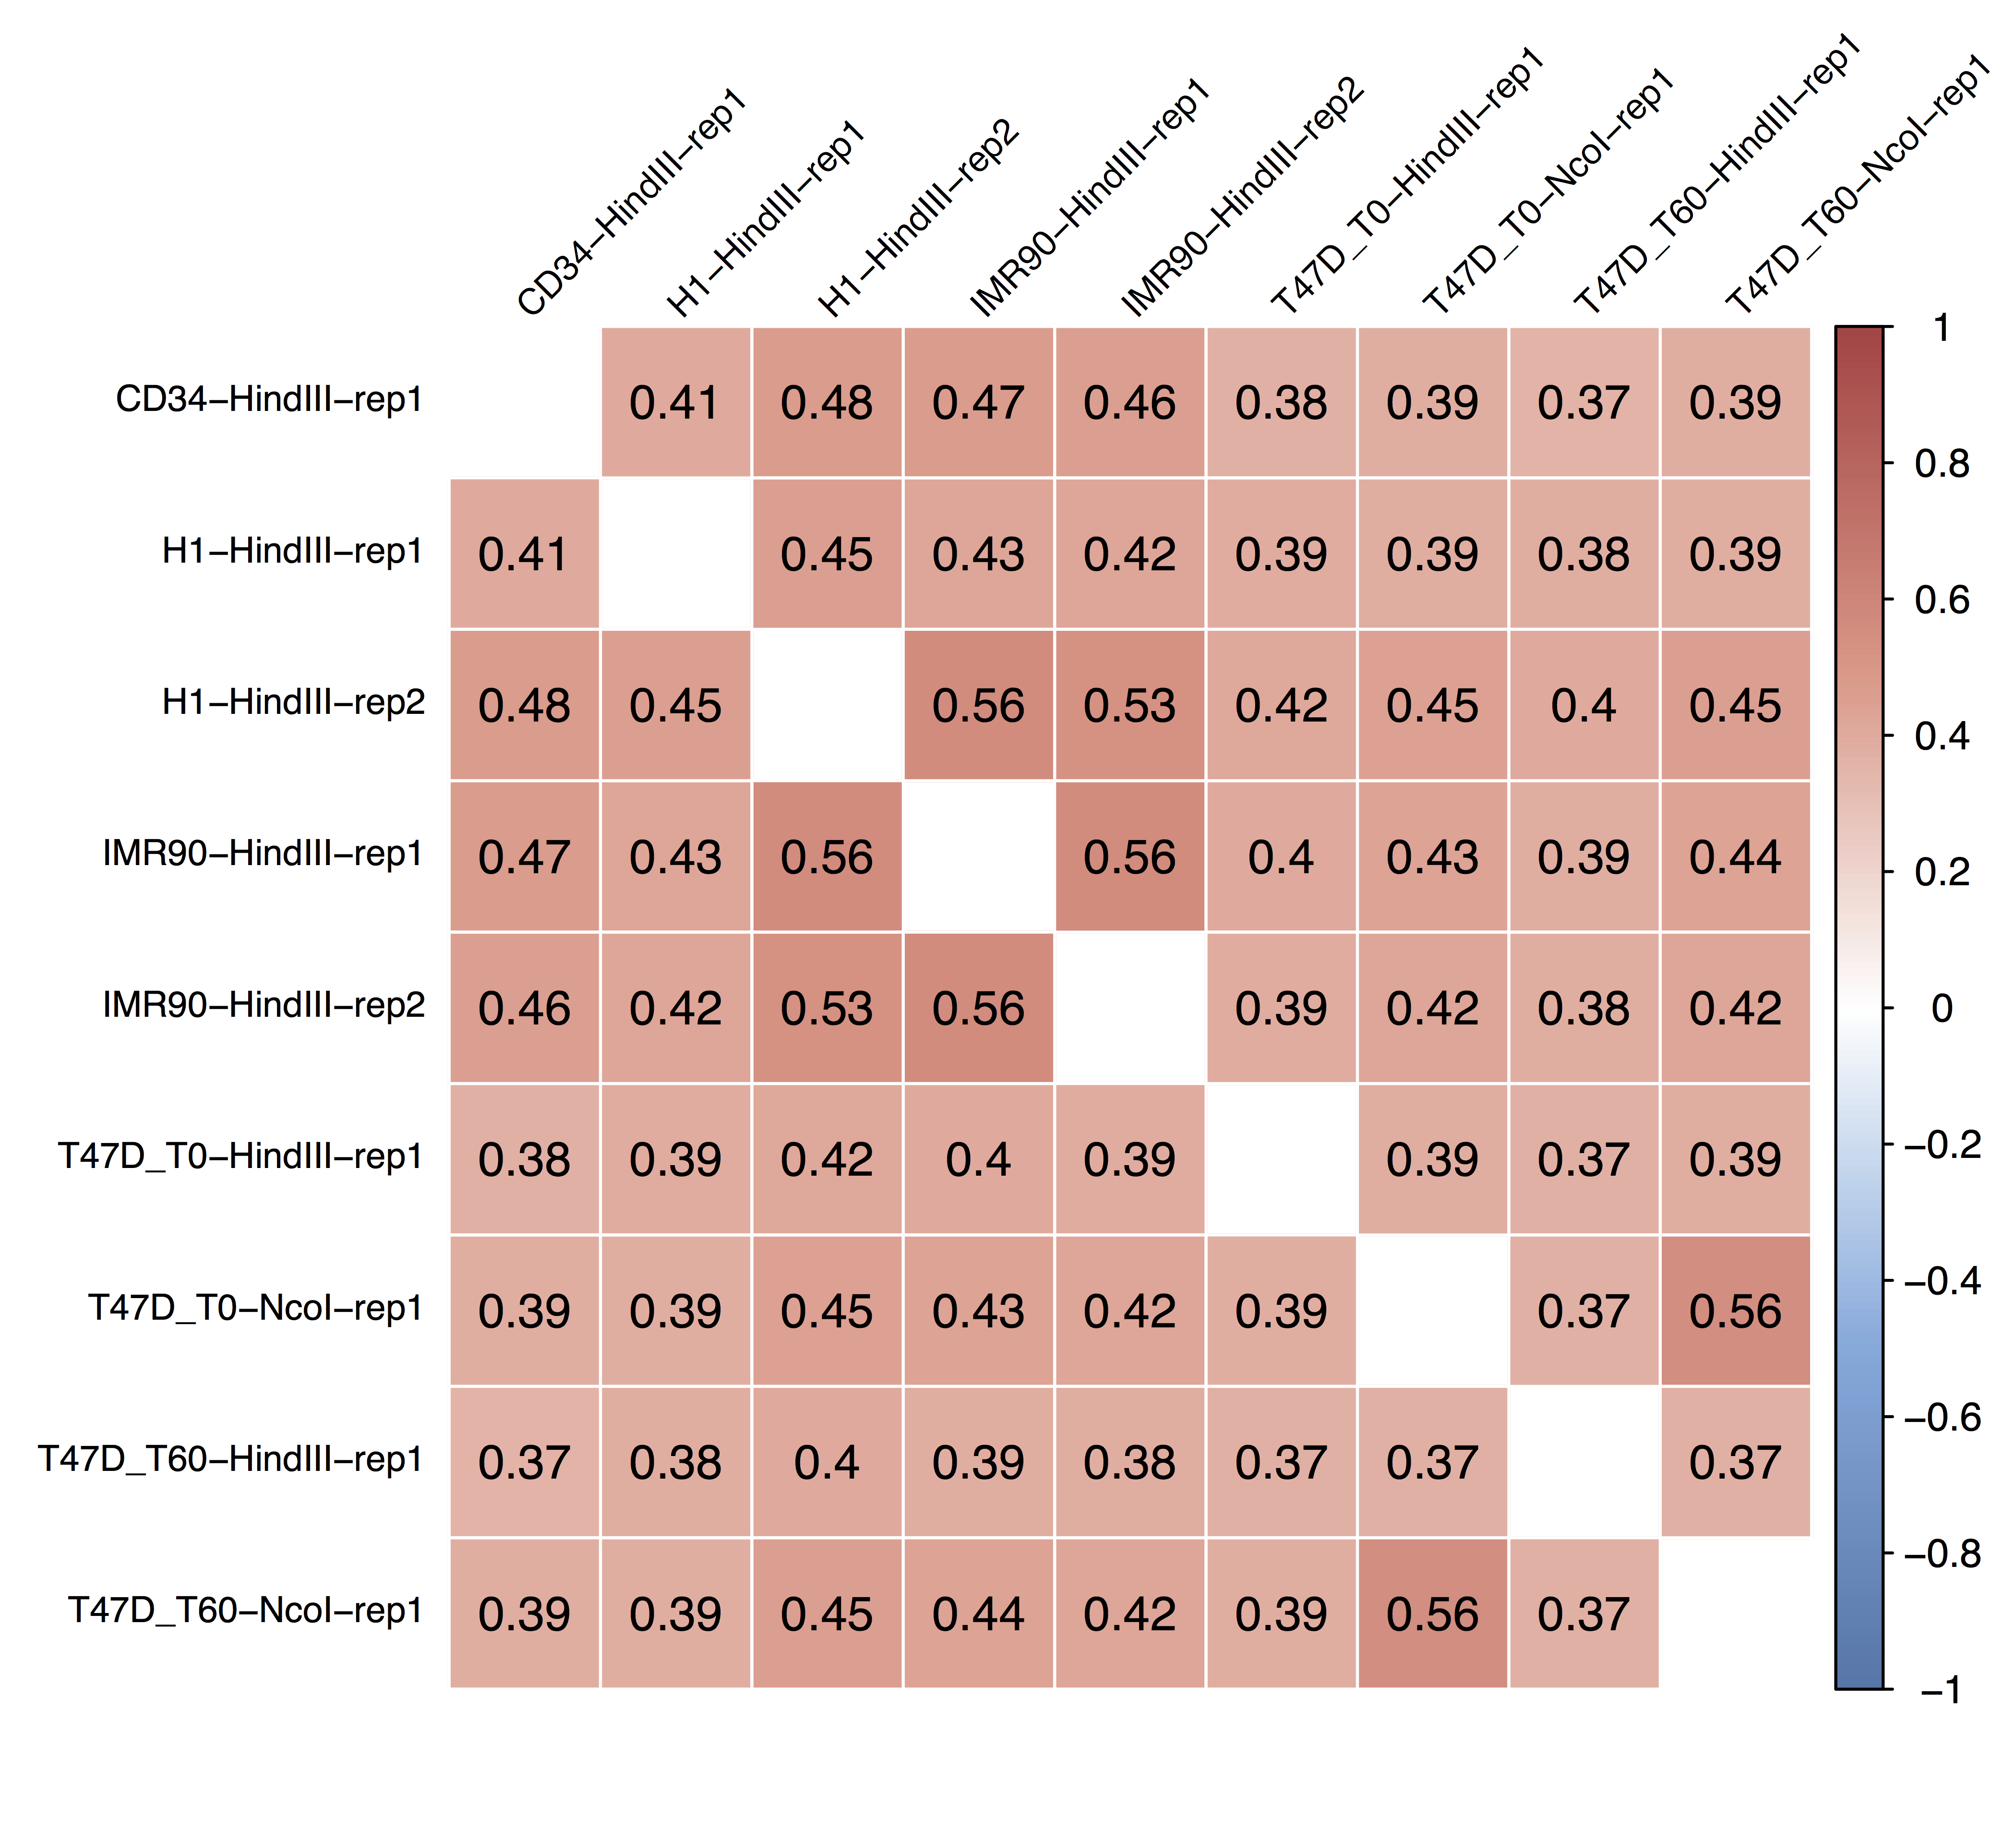
\includegraphics[width=\textwidth,height=\textheight,keepaspectratio]{figure/compare-matrices-stats_correlograms}
    \caption{Compare Matrices Stats Spearman sample correlograms. See Section~\ref{HiC:compare-matrices-stats}.} % results/compare-matrices-stats.standard/compare-matrices.by_sample.standard/matrix-filtered.by_sample.res_40kb/filter.by_sample.standard/align.by_sample.bowtie2/hg19/all-samples/spearman/correlograms.pdf
    \label{fig:compare-matrices-stats_Spearman-correlograms}
\end{figure}

% ~/projects/hic-manual-report/report-base/figure/compare-matrices-stats_pearson_correlograms.pdf
\begin{figure}[!htb]
    \centering
    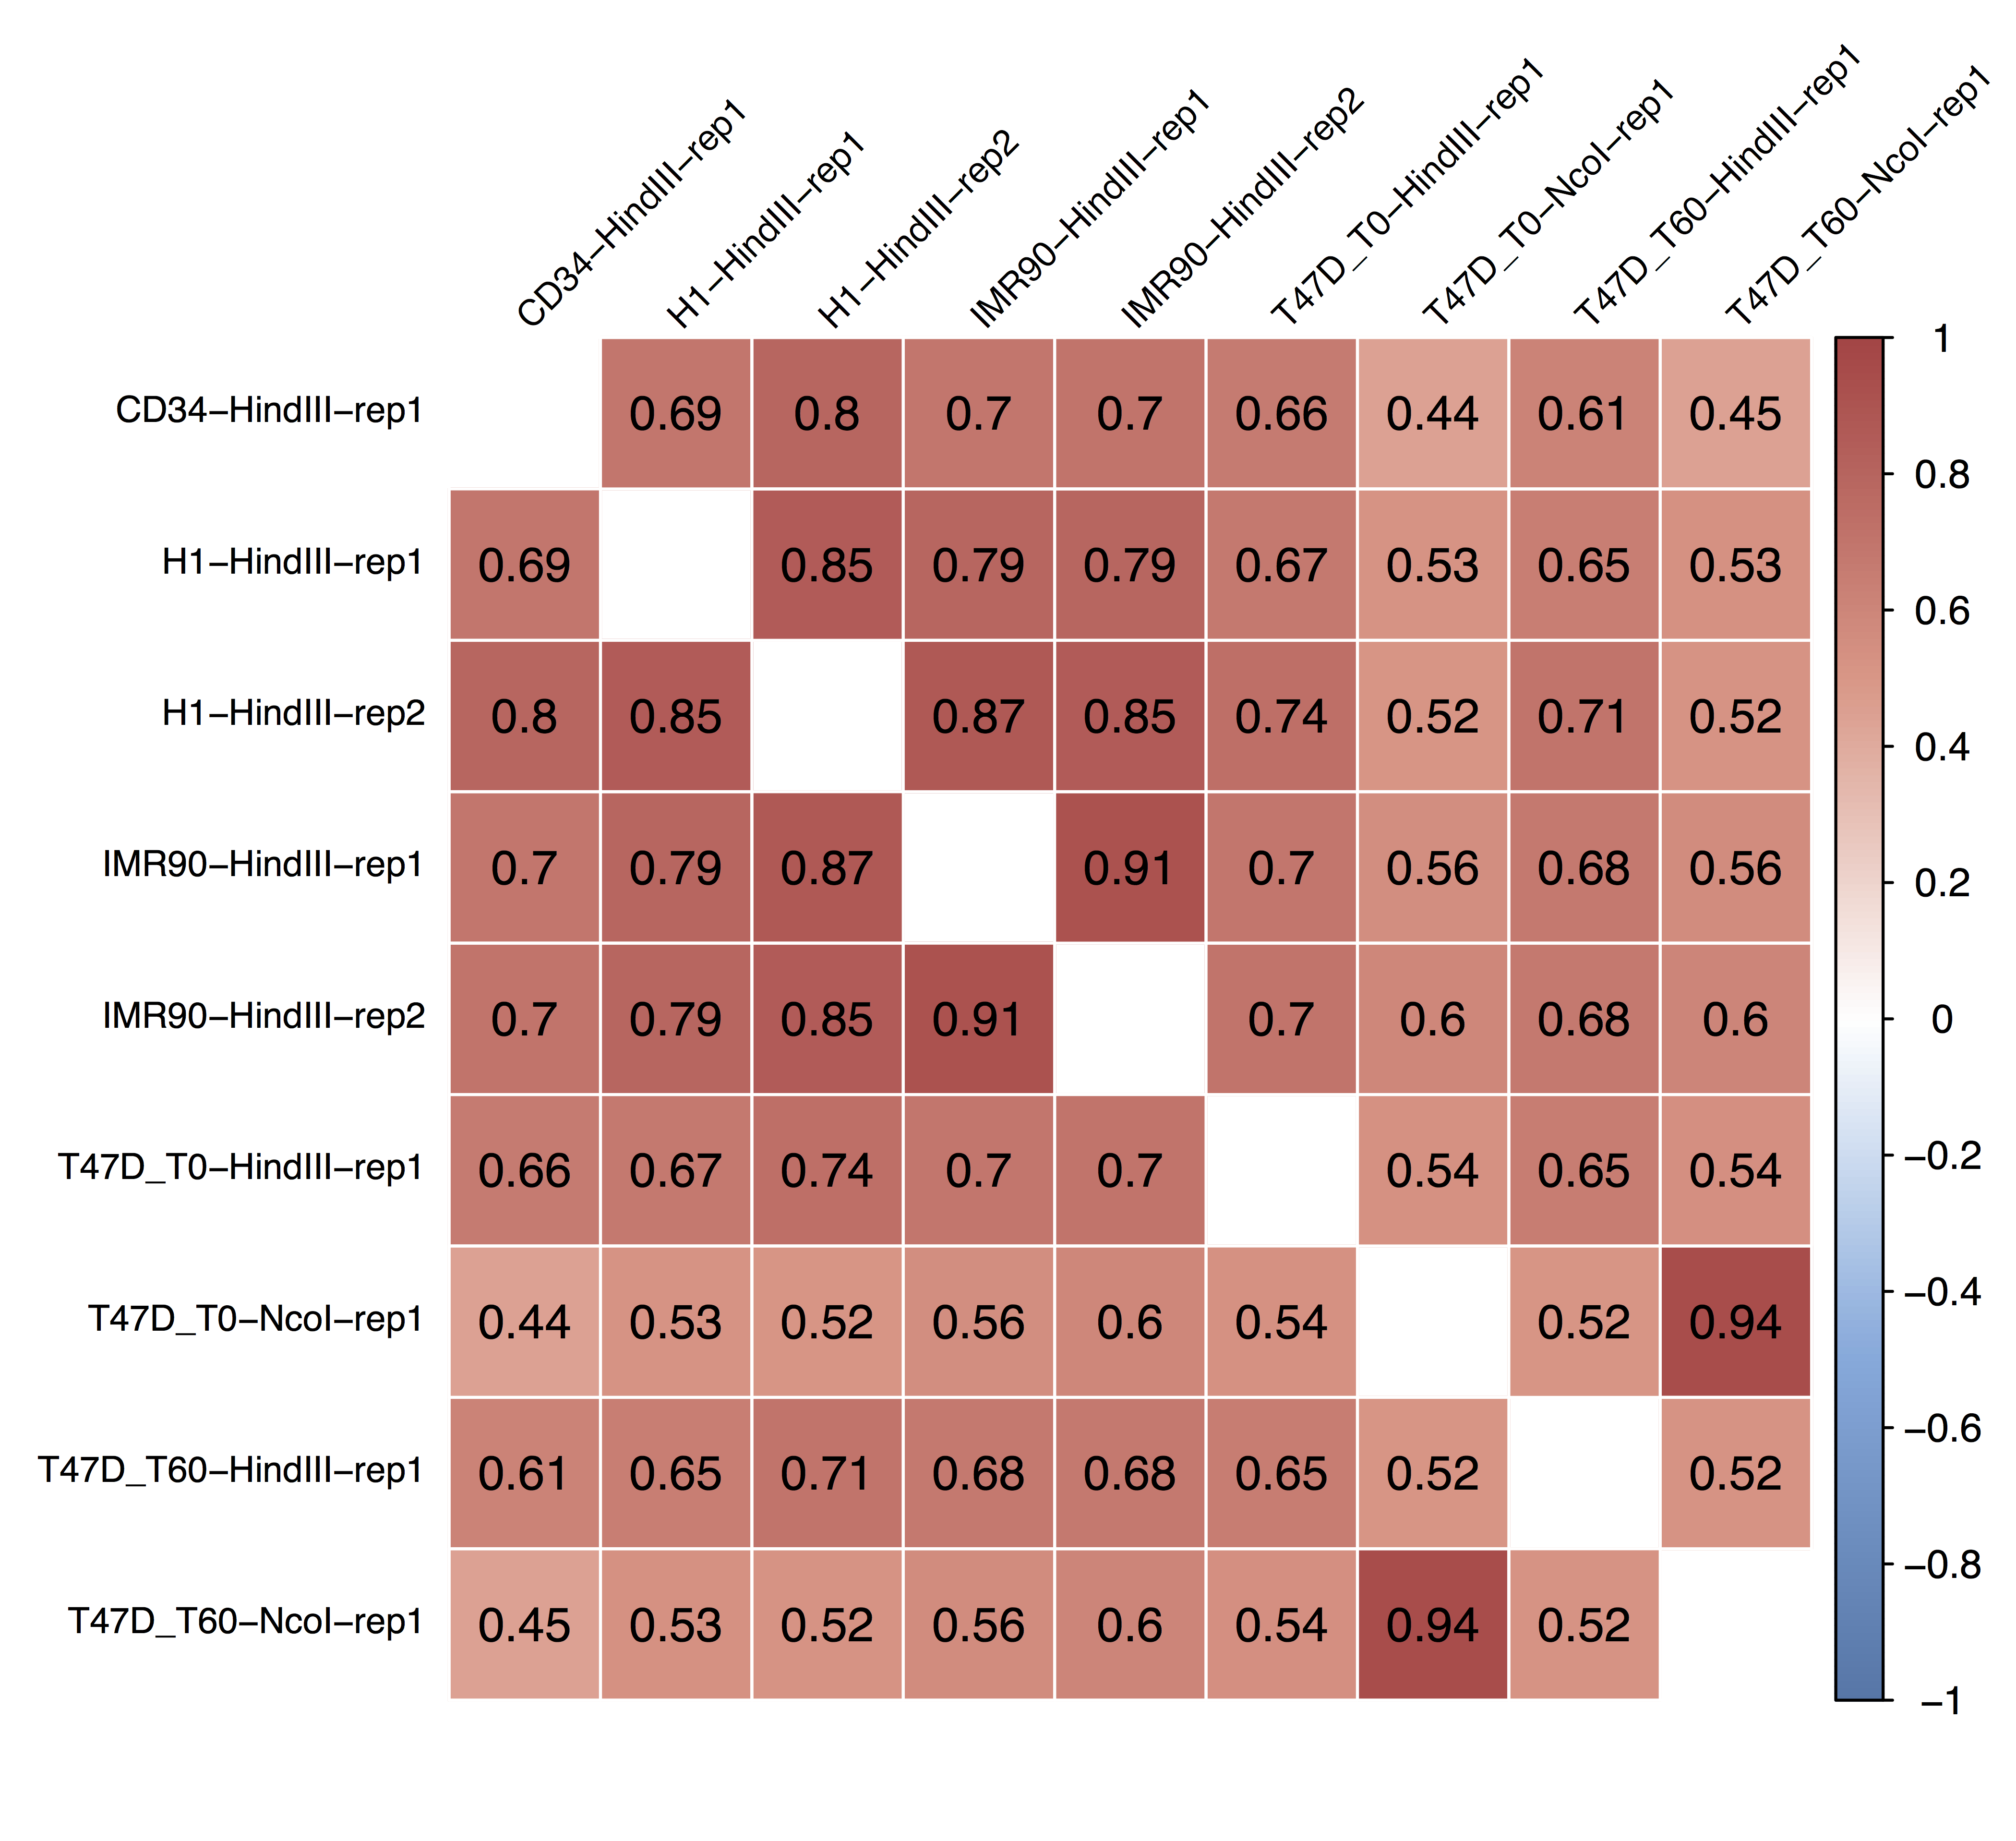
\includegraphics[width=\textwidth,height=\textheight,keepaspectratio]{figure/compare-matrices-stats_pearson_correlograms}
    \caption{Compare Matrices Stats Pearson sample correlograms. See Section~\ref{HiC:compare-matrices-stats}.} % results/compare-matrices-stats.standard/compare-matrices.by_sample.standard/matrix-filtered.by_sample.res_40kb/filter.by_sample.standard/align.by_sample.bowtie2/hg19/all-samples/pearson/correlograms.pdf
    \label{fig:compare-matrices-stats_Pearson-correlograms}
\end{figure}
% \newpage
\clearpage